% $  Id: related.tex  $
% !TEX root = main.tex


%%
\section{Background \acl{AI} Approaches}
\label{sec:related}

%%%
\subsection{Linear Regression}

Regression Models predicts continuous values. This algorithm focuses on reducing error by making accurate predictions of data. However, it is important to understand that \ac{ML} algorithms are not able to directly sense input examples. The latter means that in order to provide the model with useful inputs it is a must to create a representation of the data. Because of this, \ac{ML} and specifically Supervised learning focus on representation rather than code. 

\begin{figure}[htbp]
  \centering
  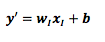
\includegraphics[width=\textwidth]{images/regresion}
  \caption{Linear Regression equation)}
  \label{fig:regresion}
\end{figure}

!!!!!!!!!!!!!!!!!!!!!!!!!!!!!Cual de los dos dejo!!!!!!!!!!!!!!!!!!!!!!!!

\begin{equation} \label{eq:linearReg}
y'=w_I x_I+b
\end{equation}

\begin{enumerate}
 \item Label (y’): is the desired output, for instance it is the target the model is aiming for.
 \item Features (x):  are the way data is represented. Because the user determines this, it is also referred to as the known input.  
 \item Weight (w):  it represents the search slope, which is the coefficient for the independent variable that in this case is the features.  
 \item Bias (b): is where the line intercepts the y-axis. It is useful because it offsets predictions made. 
 \item Subscripts (i): below each variable represents whether there is more than one dimension.
\end{enumerate}


The Model defines the connection between features and labels. In other words, it maps examples to predict labels. This is a recurrent process where it progressively learns the interrelation between features and labels. As a result the model resolves good weight and bias for all values from the given examples.  Over the fact that the user modifies the parameters of the model it is imperative to measure how far predictions are from reality.  A common way to identify the error is through the Least Square errors technique. Although there are other methods this one results attractive when the user is beginning to interact with Supervised Machine Learning because the difference between an incorrect target and the original value will be largely evident and squaring it will make it even larger. This way the errors in a single example using the model will be easier to identify, and thus more apparent to improve and modify.\fref{fig:L2loss equation} shows the equation used to calculate the Least Square errors in the model.


\begin{figure}[htbp]
  \centering
  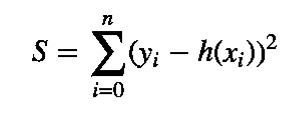
\includegraphics[width=\textwidth]{images/equation1}
  \caption{ Least Square errors equation}
  \label{fig:L2loss equation}
\end{figure}


Where h(x) represents the corresponding estimated value of x. ~\cite{rish15} 
The aim is to reach the minimum loss of the model; this goal is achievable through different approaches. For the means of this paper only two will be mentioned. The first one, known as Gradient Descent is the derivate of the least square error result and together with the weight and bias for a given example informs how loss changes for a given example. This way it is possible to adjust the model iteratively until learning weights and bias become the lowest possible. 

In the other hand there is the Stochastic Gradient Descent \ac{SGD} where the process is repeated for each individual example.

\begin{equation} \label{eq:SGD}
(y – h(x))^2
\end{equation}


In this case equation~\ref{eq:SGD} portraits the case in which the gradient is calculated one example at a time. As a result, initial values for b and w are not relevant. However most of the time it is appropriate to begin with 0 in both values.

Both Gradient descent algorithms multiply the gradient by a scalar known as the learning rate (sometimes called step size) to determine the next point.  There are several variations to the Stochastic Gradient Descent, and in all of them it is possible to set the learning rate.  Moreover, the learning rate parameter tells the optimizer how for to move the weights in the direction of the gradient for a mini batch. Having a low learning rate is decisive because it provides a more reliable training but it also means that optimization will take a lot of time because the steps towards the minimum loss of the function are especially small. In the other hand, if the learning rate is high it is possible that the training doesn’t converge and might even diverge.  Weight changes can become so big that the optimizer overshoots the minimum and makes the loss worse. The information presented before arises a new question: How can the modeler identify the correct learning rate for the process? 
As delusive as it might be, the first method with which one can select the correct learning rate is the Naïve approach. This consists of trial and error, start with any learning rate and from there start modifying it according to the received results. 

\begin{figure}[htbp]
  \centering
  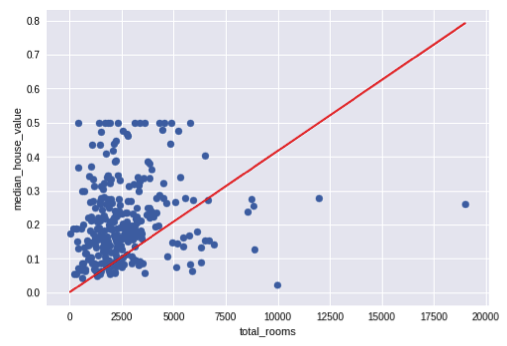
\includegraphics[width=\textwidth]{images/linearGraph}
  \caption{ The results plotted in the graph suggest that there might be a better line, which fits more data, thus resulting in a prediction model that has a greater accuracy.}
  \label{fig:linearGraph}
\end{figure}


It is recommended to start with a large value such as 0.1 and from there exponentially lower the values (0.1,0.01,0.001).
The second method created by Leslie N. Smith published in her paper Cyclical learning rates~\cite{leslie15} consists of an initial low learning rate that is then increased exponentially when a new batch comes in.

\begin{figure}[htbp]
  \centering
  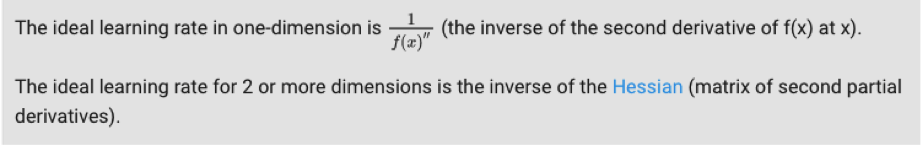
\includegraphics[width=\textwidth]{images/learningRate}
  \caption{ Ideal Learning Rates according to Leslie N. Smith (taken from~\cite{leslie15}) }
  \label{fig:learningRate}
\end{figure}


%%%%
\paragraph{Applications}



%%%
\subsection{Neural Networks}

Neural Networks \ac{NN}  are a collection of parallel processors connected together in the form of a directed graph, organized such that the network structure lends itself to the problem being considered. Scientists studied human neurons and were able to identify that the impressive parallelism and interconnectivity observed in the biological systems account for the ability of the brain to perform complex pattern recognition in a few hundred milliseconds ~\cite{freeman91}.

A biological neuron has three components important in the understanding of artificial neurons: its dendrites, soma and axon. Summed up, electric impulses known as signals are transmitted through the synaptic gap by means of a chemical process. The action of the chemical transmitter modifies the incoming signal (typically by scaling the frequency if the signals that are received) in a manner similar to the action of the weights in an Artificial Neural Network ~\cite{fausett93}. When sufficient input is received, the cell fires; that is, it transmits a signal over its axon to other cells. 

\begin{figure}[htbp]
  \centering
  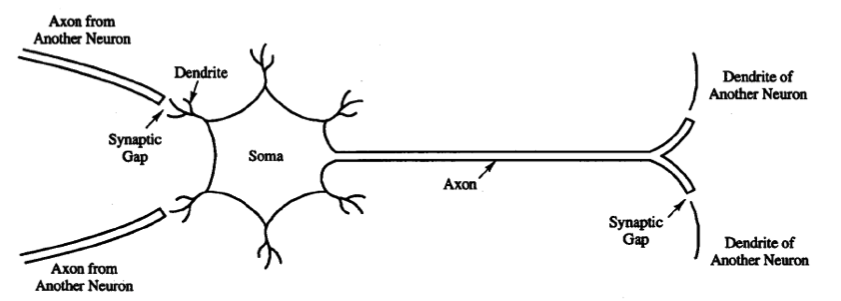
\includegraphics[width=\textwidth]{images/neuron}
  \caption{ Human Neuron diagram (taken from~\cite{fausett93}) }
  \label{fig:humanNeuron}
\end{figure}

\begin{enumerate}
 \item Axon:  region where a neuron sends messages to other neurons.
 \item Dendritic tree: area where the neuron collects input from other neurons.
 \item Synapses: in this region an axon from one neuron contacts the dendritic tree of another neuron. A Spike of activity in the axon causes charge to be injected into the post-synaptic neuron.
\end{enumerate}

According to this, Neural Networks comprise a system where biological neurons are represented by nodes and are considered a simplified representation of a processing element (unit). Additionally, connections between units are represented as arcs and this is therefore interpreted as the architecture of the model ~\cite{fausett93}. Likewise, as a way to indicate the information flow of the network arrowheads in the model are present in connections between nodes. Furthermore understanding the dynamics of the model is important to recognize how similar the Machine Learning version is to the biological nervous system. As a matter of fact, humans are born with as many as 100 billion neurons that are not replaced when they die. As a reflection of this, Neural Networks are designed to be insensitive to small damage to the network. 

When using  \ac{NN}  it is not necessary to handle correct algorithmically defined procedures that are able to take an input and represented in the correct output. Alternatively, for this type of models a collection of representative examples with the desired translation is needed. Progressively the model will adapt itself to return the desired output when presented with known inputs. As a results, \ac{NN}  have the strong characteristic of finding its  own solution to particular problems with the use of experience. 

\begin{figure}[htbp]
  \centering
  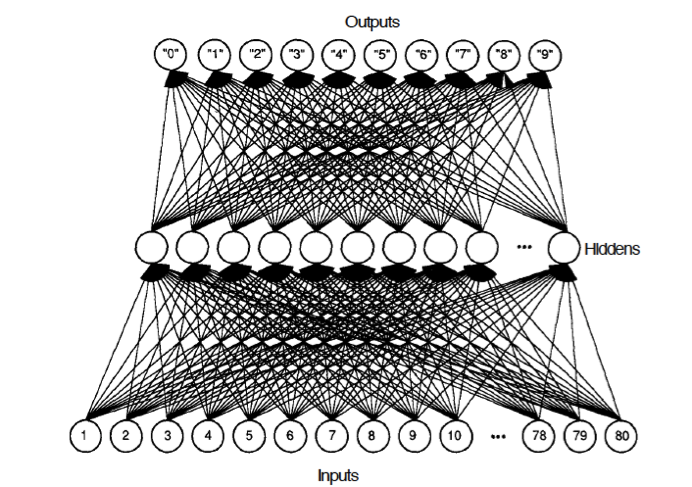
\includegraphics[width=\textwidth]{images/net}
  \caption{ Diagram of a Neural Network capable of identifying written numbers(taken from~\cite{freeman91}) }
  \label{fig:neuronNet}
\end{figure}

Neurons in these models can be classified according to the amount of detail and complexity of the inputs. Among these classifications one can find linear neurons, binary threshold neurons, rectified linear neurons, sigmoid neurons and finally stochastic binary neurons. For the means of the project implemented for this investigation, a model comprised with linear neurons was developed~\cite{hinton13}. 

Linear neurons identified as the simplest ones are good to begin with but it also implies a limited computational power.

The latter function can take any kind of scores and turn them into proper probabilities. Proper probabilities sum to one.  Results can be interpreted in the following manner: they will be large when the scores are large and small when the scores are relatively small. 
Output y is a function of a bias that is in neuron b, and the sum of all its incoming connections of the activity on an input line times the synaptic weight on that same input line. Aside from this, to identify how the model is working, there are methods that measure error such as proper probabilities. In order to turn the output, also known as scores, into probability a softmax function is needed.

\begin{figure}[htbp]
  \centering
  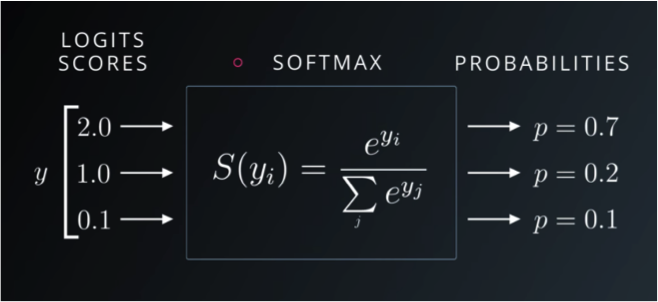
\includegraphics[width=\textwidth]{images/softmax}
  \caption{ Softmax function (taken from~\cite{hinton13}) }
  \label{fig:softmax}
\end{figure}

As seen on the \fref{fig:softmax} function, it can take any kind of scores and turn them into proper probabilities and proper probabilities sum to one.  Results can be interpreted in the following manner: they will be large when the scores are large and small when the scores are relatively small. 
%%%%
\paragraph{Applications}




\endinput

